% language.tex

\chapter{The configuration file language} \label{chap:language}
The configuration file language was designed to be a flexible and easy to use (and
learn) language that can be used to specify a user interface, file generators
and the relationship between these two.

\bigskip \noindent
The main goal of this chapter is to present and explain the language and its
features.

\bigskip \noindent
First of all, some of the more general constructions used in the language are
presented and explained in Section \ref{sect:language:structure}. Because the
configuration file describes two different phenomena (user interface
specification and technology file format specification), a certain division of
the file is to be expected. Language constructions related to the user
interface are presented in Section \ref{sect:language:uiref}. Generator
constructions are described in Section \ref{sect:language:generatorref}.

%%%%%%%%%%%%%%%%%%%%%%%%%%%%%%%%%%%%%%%%%%%%%%%%%%%%%%%%%%%%%%%%%%%%%%%%%%%%%
%%%%%%%%%%%%\section{Language features} \label{sect:language:features}

%%\bigskip \noindent
%%The configuration file will contain the information that will eventually build
%%the component tree and the generators. This means that the language should
%%support some way of structuring. The elements that need to be structured are
%%the components (the nodes in the component tree) and the nodes of the generator
%%trees that will evaluate to plain text.
%%
%%Because of this subtle difference a difference in these two parts is to be
%%expected. The main structure of the file will be discussed next, followed by
%%these two parts, the user interface reference and the generator reference.

%%%%%%%%%%%%%%%%%%%%%%%%%%%%%%%%%%%%%%%%%%%%%%%%%%%%%%%%%%%%%%%%%%%%%%%%%%%%%
\section{Language design and overview} \label{sect:language:structure}
%The configuration file will contain a user interface specification and
%generator specifications. As was explained in Chapter \ref{chap:design}, there
%is a relationship between these two because the generator specification needs
%to refer to input fields in the user interface specification. Since the
%generators depend on the user interface they are placed after the user
%interface specification.

\bigskip \noindent
\subsubsection*{A note about notation}
This chapter contains many examples in the form of source code fragments.
Source code fragments can be recognized by the
\verb=typewriter font=. Identifiers in these examples can be recognized by their
\texttt{\emph{italic}} font. Sometimes some lines have been left out for
clarity, or additional statements could be present but are not relevant for the
example. This is indicated with three dots: \verb=...=.

The language also supports C++ style comments. If two slash characters
(\verb=//=) are encountered the rest of the line is ignored.

\subsection{Structuring of components} \label{sect:language:structuring}
The parser will have to create the component tree and expression tree described
in Section \ref{sect:design:components} and \ref{sect:design:filegeneration}.
It would be helpful for the parser if the tree structure of the component and
expression trees correspond with the hierarchy in the configuration file
language. A common way to structure a language is by using hierarchical blocks.
Blocks have a start and end marker and can be nested.

For example: if we assume the block start marker is the \verb={= character and
the block end marker is the \verb=}= character we can build the tree structure
in Figure \ref{fig:language:tree_example} like this:
\begin{verbatim}
A {
    ...
    B {
        D {
            ...
        }
        E {
            ...
        }
        F {
            ...
        }
    }
    C {
        ...
    }
    ...
}
\end{verbatim}
The block start/end markers unambiguously define the tree structure from Figure
\ref{fig:language:tree_example}. The indentation (leading whitespace) used here
is only to clarify the structure, it is not mandatory. We could also have
written \verb= A {B { D {} E {} F {} } C {} }=, but this is more obscure.


\begin{figure} \begin{center}
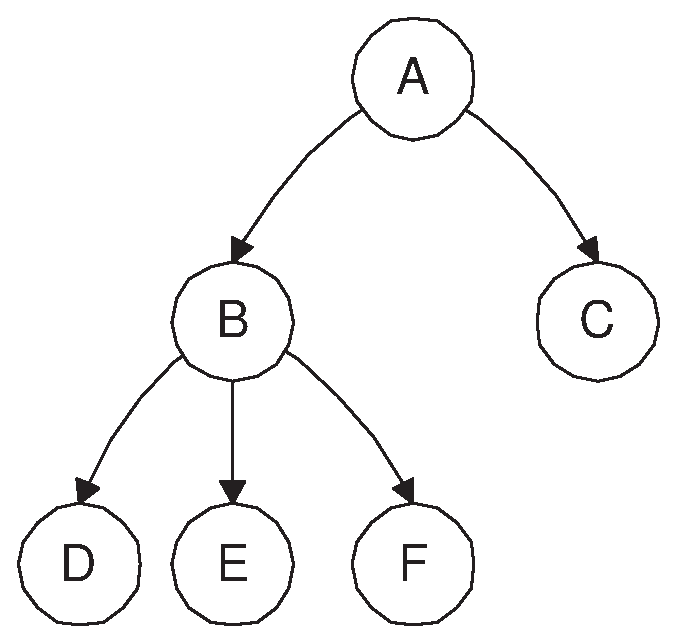
\includegraphics[width=5cm]{./figures/language_tree_example.eps}
\caption{Structuring example}
\label{fig:language:tree_example}
\end{center} \end{figure}

\bigskip \noindent
Note that the tree in Figure \ref{fig:language:tree_example} contains a
toplevel node (node A), one embedded node (node B) and several leaf nodes (D,
E, F and C). Likewise, the configuration file language distinguishes between
toplevel, embedded and leaf components. The possible components for each of
these categories are discussed in Section \ref{sect:language:uiref}.


\subsection{Component types}
As mentioned earlier, the components in the tree have type and the type
determines what kind of user interface element is created for that component. The types range
from strings and numbers to spreadsheets and sections. A common typing
mechanism is to put the type name in front of the declaration. For example, if we
were to declare an instance of \verb=spreadsheet= type named
\verb=capacitances= this would result in:
\begin{alltt}
spreadsheet \emph{capacitances} \{
    ...
\}
\end{alltt}
In this example, \verb=spreadsheet= is the type of the component and
\texttt{\emph{capacitances}} is the identifier with which this instance can be
referred to. This identifier can be used in the generator specifications to
access the values in the spreadsheet entered by the user.

This approach is very usable and is therefore applied in the configuration file
language.

\subsection{Properties}
Components support properties (see also Section \ref{sect:design:components})
and a mechanism to set the properties of a component should be present in the
language. This can be done in many ways. The obvious way would be to use the
equality sign:
\begin{alltt}
section \emph{conductors} \{
    title = "Conductors list";
\}
\end{alltt}
This approach has a disadvantage however, because this construction looks too
much like an assignment. Assignments are normally used to set the value of an
identifier. This could lead to confusion because identifiers are used to name
the components. The user could think that these identifiers can have values
assigned, for example: \verb|conductors = | \verb|"Conductor list"|. This is
not the case. In the example above \verb=title= is not an identifier that can
have a value assigned, but a property that can have a value set. It is better
to reserve the assignment construction for a future version of the language
that will support these identifier assignments.

A different construction is therefore needed to set property values. The
approach finally taken is to use rounded brackets after the property name.
Inside the brackets is the new value for the property:
\begin{alltt}
section \emph{conductors} \{
    title("Conductors list");
\}
\end{alltt}
This is a more function-like approach. Comma's can be used to add additional
values, like in the example below:
\begin{alltt}
conditionlist \emph{condlist_contacts} \{
    adddatafrom(maskdata_sheet.name, maskdata_sheet.comment);
\}
\end{alltt}
The interpretation of the property values (the ``arguments'') depend on the
context in which they are used. The possibilities are discussed in Section
\ref{sect:language:uiref}.

\subsection{Generators} \label{sect:language:generators_intro}
The technology file generator specifications do not completely ``fit'' into the component mechanism
previously described. The mechanism suffices for naming the generator and setting some
basic properties of the generator, but not for the expression tree that will
evaluate to the generated text.

Because of this, a special component statement is introduced that switches the
parser to a new mode. In this mode, each string is treated as literal text.
Identifiers that point to some part of the user interface evaluate to the value
entered by the user in that part of the user interface. For example:
\begin{alltt}
generator \emph{maskdata_gen} \{
    filename("maskdata");
    title("Maskdata file");

    generate \{
        "# Automatically generated file. Do not edit.\(\backslash\)n"
        "number_of_rows:\t" maksdata_sheet.numrows "\(\backslash\)n"
        "#############################################\(\backslash\)n"
    \}
\}
\end{alltt}
In this example, the \verb=generate= statement switches the parser to the
generator mode. The plain-text and identifier methods are also demonstrated.
Some special constructions are available as well, but these are discussed in
detail in Section \ref{sect:language:generatorref}.

\subsection{Macro definitions} \label{sect:language:macros}
In some cases it is useful if it is possible to define a macro. For example,
condition lists are used in multiple places. An example condition list is given
below:
\begin{alltt}
conditionlist \emph{condlist_simp} \{
    option("noextended");
    adddatafrom(maskdata_sheet.name, maskdata_sheet.comment);
    title("Condition list"); // Default title
\}
\end{alltt}
It would be convenient if there was a way to repeat this condition list without
retyping all properties. This is can be achieved by placing the word
\verb=define= in front of this declaration:
\begin{alltt}
define conditionlist \emph{condlist_simp} \{
    option("noextended");
    adddatafrom(maskdata_sheet.name, maskdata_sheet.comment);
    title("Condition list"); // Default title
\}
\end{alltt}
We can now use this \verb=condlist_simp= as a new component type:
\begin{alltt}
spreadsheet \emph{conductors_sheet} \{
    ...
    condlist_simp \emph{cond_list} \{
        title("Conductor condition list:"); // Overriding or
        align(right);  // adding a property is allowed.
    \}
    ...
\}

spreadsheet \emph{fets_sheet} \{
    ...
    condlist_simp \emph{cond_list} \{
        title("FET condition list:"); // Overriding a
                               // property is allowed.
    \}
    ...
\}
\end{alltt}
The three properties as defined in the macro do not have to be typed again. The
example also demonstrates the possibility to set additional properties like the
\verb=align= property. It is also possible to override a property. This is
demonstrated with the \verb=title= property.

If the \verb=title= property does not need to be redefined an empty block must
be specified with curly braces (\verb=condlist_simp cond_list {}=). To people
with programming experience this can be confusing. They would expect a
semicolon to be sufficient. However, this language construction is already used
in the ``chopping'' mechanism, and using it on a macro reference would result
in undefined behaviour. The ``chopping'' mechanism is explained in Section
\ref{sect:language:chopping}. Perhaps in a next release of the language this
behaviour could be changed.

\bigskip \noindent
Another useful application of this mechanism is in dropdowns or comboboxes. For
example, if the user can choose the accuracy of an algorithm and there are many
algorithms to run:
\begin{alltt}
define dropdown \emph{algo_acc} \{
    item \emph{highest} \{ title("Highest accuracy - longest runtime"); \}
    item \emph{high}    \{ title("High accuracy - long runtime"); \}
    item \emph{normal}  \{ title("Normal accuracy - normal runtime"); \}
    item \emph{low}     \{ title("Low accuracy - short runtime"); \}
    item \emph{lowest}  \{ title("Lowest accuracy - shortest runtime"); \}
\}

paramlist \emph{algo_params} \{
    algo_acc \emph{alg_A} \{ title("Algorithm A accuracy:"); \}
    algo_acc \emph{alg_B} \{ title("Algorithm B accuracy:"); \}
    ...
\}
\end{alltt}
This mechanism could also be used for yes/no or on/off dropdowns. One could
argue that these kind of macros should be built-in in the language. The choice
was made not to do this. This is the first version of the language and it has not
been released to a large public. The interface should therefore be kept as
clean as possible. A future version of the language could easily implement
these built-ins if the need for them arises.

\bigskip \noindent
Nesting of macros is allowed. This means it is possible to use a defined type
inside another macro.

\bigskip \noindent
\paragraph{Implementation\\ }
\noindent Whenever the parser encounters a situation in which a previously declared
\verb=define= is used, it copies the branch of the component tree of the
\verb=define= to the correct location. If any properties were added or changed
like in the first example it updates the copied branch of the component tree to
reflect these changes.

Note that the parser performs on-the-fly disambiguation for macro definitions.
This means a macro must be defined before it is used.

\subsection{Reducing indentation} \label{sect:language:chopping}
As was mentioned earlier, indentation with whitespace is not necessary. However, it
is encouraged because it increases the readability of the configuration file.
If the number of nestings becomes too large though, this readability can decrease again. The
indentation then becomes too large.

To counter this effect, a ``chopping'' mechanism is introduced. Chopping makes
it possible to place declarations outside the hierarchy if desired. For
example, a tabpage usually consists of a scrollframe with several sections:
\begin{alltt}
tabpage \emph{element_definition} \{
    scrollframe \emph{element_def_frame} \{
        section \emph{fets} \{
            spreadsheet \emph{fets_sheet} \{
                ...
            \}
            ...
        \}
        section \emph{bjts} \{
            spreadsheet \emph{bjts_sheet} \{
                ...
            \}
            ...
        \}
        ...
    \}
\}
\end{alltt}
Even in this little example the indentation becomes considerable. The
``chopping'' mechanism is demonstrated below:
\begin{alltt}
section \emph{fets} \{
    spreadsheet \emph{fets_sheet} \{
        ...
    \}
    ...
\}

section \emph{bjts} \{
    spreadsheet \emph{bjts_sheet} \{
        ...
    \}
    ...
\}

tabpage \emph{element_definition} \{
    scrollframe \emph{element_def_frame} \{
        section \emph{fets};
        section \emph{bjts};
        ...
    \}
\}
\end{alltt}
This way, the tabpage declaration remains clear because the finer details are
``hidden'' in the sections.

This method is called ``chopping'' because a branch of the component tree is
cut off, leaving a reference at the location the chopping occurred.

\subsubsection*{Differences with macro definitions}
The main differences are listed below:
\begin{itemize}
\item References to macros can be used many times. References to a chopped branch
can be used only once. If used more than once, the resulting behaviour is
undefined.
\item References to chopped branches use a different syntax than references to
defined macros. A reference to a define macro uses the macro name and must be
followed by block markers (\{ ... \}). A reference to a chopped branch must be
followed by a semicolon. If a reference to a branch is followed by block
markers the resulting behaviour is undefined. If a reference to a macro is
followed by a semicolon the resulting behaviour is undefined. As was mentioned
in Section \ref{sect:language:macros}, the syntactical difference between an
empty macro (no additions or overrides, \verb={ }=) and a chopped bracn can be
confusing for experienced programmers. However, it should be noted that chopped
branches cannot have additional or overridden properties. Hence, there is no
need for curly braces and a semi-colon suffices. In the case of a macro without
added or overridden properties, the empty curly braces indicate that something
\emph{could} be changed if desired.

As was already mentioned in Section \ref{sect:language:macros}, changing the
syntax of these constructions should be considered in a next release.
\end{itemize}

\bigskip \noindent
Like the macro definition, nested choppings are allowed. This means that in the
example it is allowed to chop the \texttt{scrollframe
\emph{element\_def\_frame}} as well.

\subsubsection*{Implementation}
If we look at it from a tree perspective, defined macro branches are
\emph{copied} to new locations in the tree while the chopped of branches are
\emph{moved} back to the position where they belong. This is done by
the parser. Whenever the parser encounters a reference to a chopped of branch,
it tries to find the chopped of branch and moves it to the correct position in
the component tree.

Note that the parser performs on-the-fly disambiguation for chopped branches,
just like it does for macro definitions. This means the chopped branch must be
put before the reference to it.

\subsection{Data connections}
The data connections as discussed in Section \ref{sect:design:dataconnections}
must have a place in the language as well. A data connection consist of one or
more sources linked to a single target. Therefore, the most logical place to
define a data connection would be inside the target component. If we make a
data connection declaration a property, we can also use the
\verb=CFindPropertyVisitor= class to find them when the data connections need
to be built. An example of the implemented construction is given below:
\begin{alltt}
define dropdown \emph{layer} \{
    adddatafrom(maskdata_sheet.name, layer_synonyms.name);
\}
\end{alltt}
In this example we define a dropdown \verb=layer=. The items in the dropdown
are the \verb=name= column in the spreadsheet \verb=maskdata_sheet= and the
spreadsheet \verb=layer_synonyms=.

The data connections are established right after the \verb=CGUITree= object is
created by the \verb=CGUIBuilderVisitor=.

\bigskip \noindent
The only datasource currently implemented is a column in a spreadsheet. The
currently available data targets can be found in the \verb=adddatafrom= column
of Table \ref{tab:language:overview}.

%\begin{table}[t!]
%\caption{Data targets. Components not present in this table do not support the
%\texttt{adddatafrom} property. }
%\label{tab:language:data_connections}
%\begin{tabular}{l|p{25mm}|p{55mm}}
%\hline
% \textsf{Context} & \textsf{Possible target components} & \verb=adddatatfrom= \textsf{arguments} \\
%\hline
%\verb=spreadsheet=  & \verb=dropdown,= \verb=combobox=  &  Each argument is the unambiguous name of a valid data source.
%                                                             Each cell in the column described by the dropdown or combobox
%                                                             will have the values of the sources specified in the
%                                                             \verb=adddatafrom= argument. The number of arguments (sources)
%                                                             allowed is one or more. The data obtained from the sources is
%                                                             concatenated.\\
%                    & \verb=conditionlist=                & The first argument defines the source for the layer names.
%                                                            The second argument
%                                                            defines the source
%                                                            for the layer
%                                                            descriptions. The first argument is required, the second is optional.\\
%non-spreadsheet   &  \verb=dropdown,= \verb=combobox=  &  Each argument is the
%unambiguous name of a valid data source.
%                                                             The dropdown or combobox will have the values of the sources
%                                                             specified in the \verb=adddatafrom= argument. \\
%\hline
%\end{tabular}
%\end{table}

%%%%%%%%%%%%%%%%%%%%%%%%%%%%%%%%%%%%%%%%%%%%%%%%%%%%%%%%%%%%%%%%%%%%%%%%%%%%%
\section{Language overview for user interface elements
\label{sect:language:uiref}}
This section will present all the component types that can be used to create a
user interface. The context in which a certain component type is used
determines what kind of user interface element is created. The context also
affects how a component's properties are used.

Since the context largely determines what will happen, the descriptions of the
component types and their properties are given relative to the context in which
they can be used.

As was mentioned in Section \ref{sect:language:structuring}, we can distinguish
between toplevel, embedded and leaf components. Table
\ref{tab:language:top_leaf} lists which component types belong to which
category.

\begin{table} \begin{center}
\caption{Classification of components.}
\label{tab:language:top_leaf}
\begin{tabular}{l|p{6cm}}
\hline
 \textsf{Classification} & \textsf{Component type(s)} \\
\hline
toplevel     & \verb=tabpage= \\
embedded     & \verb=dropdown,= \verb=combobox,= \verb=spreadsheet,= \verb=section,= \verb=paramlist,= \verb=scrollframe=  \\
leaf         & \verb=integer,= \verb=real,= \verb=string,= \verb=identifier,= \verb=conditionlist=, \verb=color,= \verb=dalistyle=, \verb=item= \\
\hline
\end{tabular} \end{center} \end{table}

The components that can provide a context are the top level and embedded
components. Leaf components cannot provide context, but their interpretation
strongly depends on the context in which they are used.

\bigskip \noindent
In the following subsections, all the context-providing component types are
presented. The interpretation of the components inside the context being
discussed is explained in these subsections. Small examples with their
resulting user interface are given as well. At the end of this section, a
complete overview of the currently possible combinations of context, component
types and properties is presented in Table \ref{tab:language:overview}

\bigskip \noindent
\textbf{Note:} Although it is possible to place components \emph{visually} on
the top level (because of the chopping mechanism described in Section
\ref{sect:language:chopping}), the components \emph{as seen after parsing}
still adhere to the classification presented in Table
\ref{tab:language:top_leaf}.

%\subsection{Leaf components}
%The leaf components can be divided into numbers (\verb=real= and
%\verb=integer=), text types (\verb=string=, \verb=identifier=,
%and \verb=conditionlist=) and color/fill style types (\verb=color= and
%\verb=dalistyle=). The actual widget that will be created for them depends on
%the context in which they are found. Also, not every context is applicable. For
%example, when a \verb=string= is encountered inside a \verb=paramlist= the
%widget will be a \verb=QLineEdit=. If it is encountered inside a spreadsheet,
%it will become a column of that spreadsheet.

\subsection{Components in a dropdown or combobox context }
The dropdown is used exactly the same as the combobox. The only difference is
in the behaviour of the widget that will be created. Dropdown widgets present
the user with a fixed list of choices. The combobox widget also presents a list
of choices. However, the user can also enter text not present in the list of
available choices. Because of the similarities we will only discuss the
dropdown.

\bigskip \noindent
The dropdown can only have \verb=item= children inside. All items will become
entries in the dropdown widget. Each item must have the \verb=title= property
set to the text that will be displayed as the entry in the dropdown widget. If
the \verb=title= property of an item is not specified, an empty entry will be
inserted in the dropdown.
%%%\small
%%%\begin{center}
%%%\begin{tabularx}{\textwidth}{|l|l|X|}
%%%  \hline
%%%  \multicolumn{3}{|l|}{\textsf{List of accepted child components}} \\
%%%  \hline
%%%  \multicolumn{3}{|l|}{Child component type: \texttt{item}} \\
%%%  \hline
%%%  &  \textsf{Property} & \textsf{Description} \\
%%%  \cline{2-3}
%%%  & \texttt{title} & The value of this property will be used as the text of the corresponding entry in the  dropdown. \\
%%%  \cline{2-3}
%%%  & \multicolumn{2}{|X|}{Ignored properties: \mbox{\texttt{hint, default, align, unit, pixmap, option}}} \\
%%%  \cline{2-3}
%%%  & \multicolumn{2}{|X|}{Forbidden properties: \texttt{adddatafrom}} \\
%%%
%%%  \hline
%%%  \multicolumn{3}{|X|}{Using forbidden properties or unlisted component types as children will result in undefined behaviour.} \\
%%%  \hline
%%%\end{tabularx}
%%%\end{center}
%%%\normalsize

\paragraph{Example:}
\begin{alltt}
dropdown \emph{def_carr_type} \{
    item \emph{n} \{ title("n doped conductor"); \}
    item \emph{p} \{ title("p doped conductor"); \}
    item \emph{m} \{ title("metal"); \}
    default(\emph{m});
\}
\end{alltt}

\begin{figure}[h!] \begin{center}
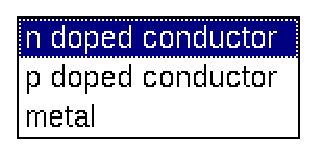
\includegraphics[width=3cm]{./figures/ex_dropdown.eps}
\caption{Dropdown example result.}
\end{center} \end{figure}


%
%\begin{PropTable}
% \verb=default=     & Sets the item that will be displayed by default.  \\
% \verb=hint=        & Sets the hint text that will be displayed when the mouse
%                      hovers over the widget. \\
% \verb=adddatafrom= & Sets this components data sources. Items received from
%                      the source will be added to this dropdown.
%\end{PropTable}

\subsection{Components in a spreadsheet context}
In a spreadsheet, each child is interpreted as a column. The number of rows
changes dynamically, as the user can add or remove rows. The edit mode of the
column corresponds to the columns type. This means a
\verb=string= column corresponds to a \verb=QLineEdit= as edit widget. These
are the types that can be columns in a spreadsheet:
\begin{itemize}
\item \verb=string=, \verb=real=, \verb=integer= and \verb=identifier=
correspond to a column using \verb=QLineEdit= widgets.
\item \verb=color= columns create \verb=CColorCells= that bring up the \verb=QColorDialog= box. They display
the selected color.
\item \verb=dalistyle= columns are edited using the dali colorpicker dialog.
The selected style is displayed in the cells.
\item \verb=conditionlist= columns are edited with the condition list editor.
\item \verb=dropdown= and \verb=combobox= columns display a dropdown
respectively a combobox widget.
\end{itemize}

\paragraph{Example:}
\begin{alltt}
spreadsheet \emph{maskdata_sheet} \{
    integer             \emph{ID} \{ title("Layer ID"); \}
    identifier          \emph{name} \{ title("Layer name"); \}
    def_layer_type      \emph{layertype} \{ title("Layer type"); \} // def_layer_type is a macro
    dalistyle           \emph{dali} \{ title("Dali draw style"); \}
    color               \emph{xspace} \{ title("XSpace draw color"); \}
    string              \emph{comment} \{ title("Comment"); \}
\}
\end{alltt}

\begin{figure}[h!] \begin{center}
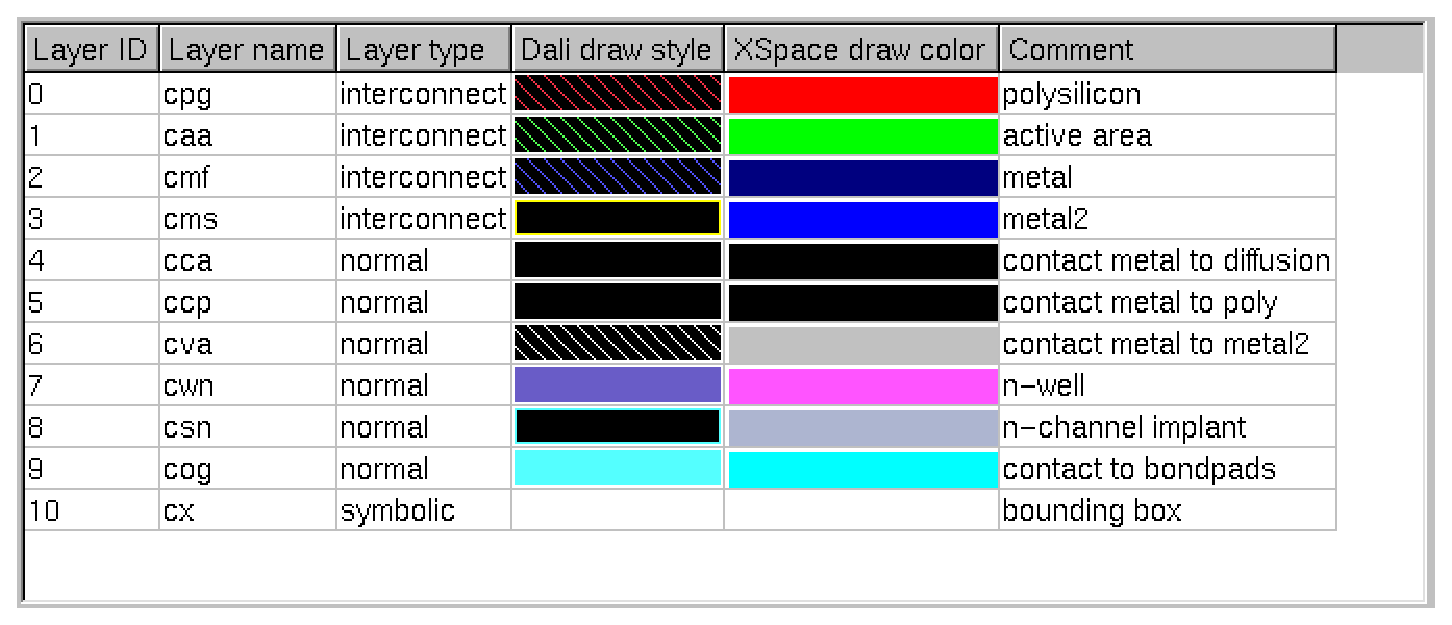
\includegraphics[width=8cm]{./figures/ex_spreadsheet.eps}
\caption{Spreadsheet example result.}
\end{center} \end{figure}

%%%\small
%%%\begin{center}
%%%\begin{tabularx}{\textwidth}{|l|l|X|}
%%%  \hline
%%%  \multicolumn{3}{|X|}{\textsf{List of accepted child components}} \\
%%%  \hline
%%%  \multicolumn{3}{|X|}{Child component type: \texttt{real, integer, identifier, string, color, dalistyle}} \\
%%%  \hline
%%%
%%%  &  \textsf{Property} & \textsf{Description} \\
%%%  \cline{2-3}
%%%  & \texttt{title} & The value of this property will be used as the title of the corresponding column in the spreadsheet. \\
%%%  \cline{2-3}
%%%  & \texttt{default} & The value of this property will be used as default value to display in the spreadsheet cells of this column. \\
%%%  \cline{2-3}
%%%  & \texttt{align} & The value of this property can be \texttt{left, right} or \texttt{center}. This column will be aligned accordingly.\\
%%%  \cline{2-3}
%%%  & \multicolumn{2}{|X|}{Ignored properties: \texttt{hint, unit, pixmap, option}} \\
%%%  \cline{2-3}
%%%  & \multicolumn{2}{|X|}{Forbidden properties: \texttt{adddatafrom}} \\
%%%  \hline
%%%
%%%  \multicolumn{3}{|l|}{Child component type: \texttt{dropdown, combobox}} \\
%%%  \hline
%%%  &  \textsf{Additional properties} & \textsf{Description} \\
%%%  \cline{2-3}
%%%  & \texttt{adddatafrom} & The value of this property should be a reference to a data source. The source data will be used to fill the dropdown.\\
%%%  \cline{2-3}
%%%  & \texttt{default} & The value of this property must be the name of an \texttt{item} child of the dropdown. \\
%%%  \cline{2-3}
%%%  & \multicolumn{2}{|X|}{Ignored properties: \texttt{hint, unit, pixmap, option}} \\
%%%  \hline
%%%
%%%  \multicolumn{3}{|X|}{Child component type: \texttt{conditionlist}} \\
%%%  \hline
%%%  &  \textsf{Additional properties} & \textsf{Description} \\
%%%  \cline{2-3}
%%%  & \texttt{adddatafrom} & Accepts two property values. They must be references to a data source. The first value of this property will be used as the condition list layer names. This value is mandatory. The second value of this property will be used for the layer descriptions and is optional. The layer descriptions are used as explanation of the (short) layer names. If the first property value is not specified, the behaviour is undefined.\\
%%%  \cline{2-3}
%%%  & \texttt{option} & The value of this property can be either \verb=extended= or \verb=noextended=. Using verb=extended= shows the condition list dialog with three columns: `one side', `tile' and 'other side'. Using \verb=noextended= will only show the `tile' column.\\
%%%  \cline{2-3}
%%%  & \multicolumn{2}{|X|}{Ignored properties: \texttt{hint, unit, pixmap, option}} \\
%%%  \hline
%%%
%%%  \multicolumn{3}{|X|}{Using forbidden properties or unlisted component types as children will result in undefined behaviour.} \\
%%%  \hline
%%%\end{tabularx}
%%%\end{center}
%%%\normalsize

%\begin{PropTable}[Description of useful child properties:]
% \verb=title=       & Use the \verb=title= property to set the column title. \\
% \verb=align=       & Use the \verb=align= property to set the alignment of the
%                      column. Possible values are \verb=left=, \verb=right= and \verb=center=. \\
% \verb=adddatafrom= & Only available if the child supports data connections.
%\end{PropTable}
%\clearpage

\subsection{Components in a paramlist context}
The parameter list displays a three column widget. The first column contains
descriptions of the input fields, the middle column contains the input widgets
and the last column can contain additional text, for example to display the
unit of the value that must be entered.

The children of the \verb=paramlist= component can be any type. The most useful
types are the \verb=string=, \verb=real=, \verb=integer=, \verb=dropdown= and
\verb=combobox= types.

%%%\small
%%%\begin{center}
%%%\begin{tabularx}{\textwidth}{|l|l|X|}
%%%  \hline
%%%  \multicolumn{3}{|X|}{\textsf{List of accepted child components}} \\
%%%  \hline
%%%
%%%  \multicolumn{3}{|X|}{Child component type: \texttt{real, integer, identifier, string, spreadsheet}} \\
%%%  \hline
%%%  &  \textsf{Property} & \textsf{Description} \\
%%%  \cline{2-3}
%%%  & \texttt{title} & The value of this property will be used as the label in the first column. \\
%%%  \cline{2-3}
%%%  & \texttt{hint} & The value of this property will be shown as a hint text as the mouse ``hovers'' over the widget in the second column. The hint text can be split over multiple lines by inserting $\backslash$n at the right places. \\
%%%  \cline{2-3}
%%%  & \texttt{default} & The value of this property will be used as the default value to display in the widget (ignored for spreadsheets). \\
%%%  \cline{2-3}
%%%  & \texttt{unit} & The value of this property will be used as the label in the third column. \\
%%%  \cline{2-3}
%%%
%%%  & \multicolumn{2}{|X|}{Ignored properties: \mbox{\texttt{align, pixmap, option}}} \\
%%%  \cline{2-3}
%%%  & \multicolumn{2}{|X|}{Forbidden properties: \texttt{adddatafrom}} \\
%%%  \hline
%%%
%%%  \multicolumn{3}{|l|}{Child component type: \texttt{dropdown}} \\
%%%  \hline
%%%  &  \textsf{Additional properties} & \textsf{Description} \\
%%%  \cline{2-3}
%%%  & \texttt{adddatafrom} & The value of this property is a reference to the data source. The data from the source is used as the entries in this dropdown. \\
%%%  \cline{2-3}
%%%  & \texttt{default} & The value of this property must be the name of an \texttt{item} child of the dropdown. \\
%%%  \cline{2-3}
%%%
%%%  & \multicolumn{2}{|X|}{Ignored properties: \mbox{\texttt{align, pixmap, option}}} \\
%%%  \cline{2-3}
%%%
%%%  \hline
%%%  \multicolumn{3}{|X|}{Using forbidden properties or unlisted component types as children will result in undefined behaviour.} \\
%%%  \hline
%%%\end{tabularx}
%%%\end{center}
%%%\normalsize

%\begin{PropTable}[Description of useful child properties:]
% \verb=title=       & Use the \verb=title= property to set the text in the first
%                      column. \\
% \verb=unit=        & Use the \verb=unit= property to set the text in the last
%                      column. \\
% \verb=hint=        & Sets the hint text that will be displayed when the mouse
%                      hovers over the widget. \\
% \verb=adddatafrom= & Only available if the child supports data connections.
%\end{PropTable}

\paragraph{Example:}
\begin{alltt}
paramlist \emph{units_list} \{
    real \emph{resistance} \{
        title("Sheet resistance unit:");
        unit("in ohm");
        hint("You can specify a base for the values you \(\backslash\)n"
             "will enter below. Use as follows:\(\backslash\)n"
             "If you do not want to type 3e-6, 8e-6 12.5e-6, etc.\(\backslash\)n"
             "but 3, 8, 12.5 instead, type 1e-6 here.");
    \}
    dropdown \emph{accur} \{
        title("Accuracy:");
        item \emph{low} \{ title("Low accuracy"); \}
        item \emph{normal} \{ title("Normal accuracy"); \}
        item \emph{high} \{ title("High accuracy"); \}
        default(\emph{normal});
    \}
\}
\end{alltt}

\begin{figure}[h!] \begin{center}
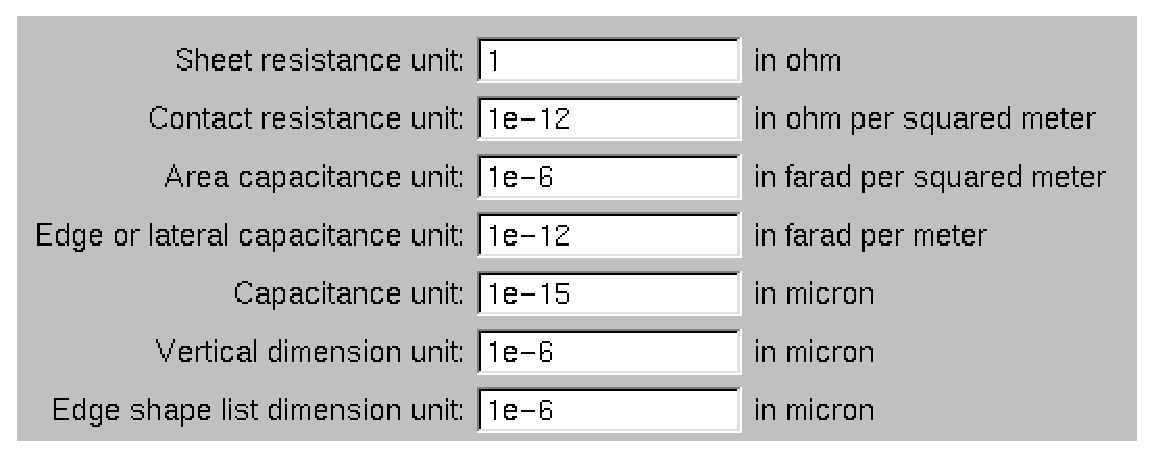
\includegraphics[width=8cm]{./figures/ex_paramlist.eps}
\caption{Parameter list example result.}
\end{center} \end{figure}


%\subsection{Condition list components}
%A condition list component can only be used inside a spreadsheet. The edit mode
%of this type of cell brings up the condition list editor. The condition list
%editor is described in Section \ref{sect:uidesign:conditionlist}.
%
%The condition list component relies on two properties: \verb=adddatafrom= and
%\verb=option=. They are described in the table below.
%\begin{PropTable}[Condition list component properties]
% \verb=title=       & Use the \verb=title= property to set the column title. \\
% \verb=align=       & Use the \verb=align= property to set the alignment of the
%                      column. Possible values are \verb=left=, \verb=right= and \verb=center=. \\
% \verb=adddatafrom= & The first data source specified is used for the layer
%                      names. It must be set for the editor to make sense. The
%                      second data source is used for the layer descriptions and
%                      is optional. \\
% \verb=options=     & The options property can be set to \verb="noextended"= or
%                      to \verb="extended"=. If option extended is specified, the
%                      editor will display the ``one side'' and ``other'' side
%                      button columns.
%\end{PropTable}
%
%\paragraph{Example:}
%\begin{alltt}
%define conditionlist \emph{condlist_ext} \{
%    option("extended");
%    adddatafrom(maskdata_sheet.name, maskdata_sheet.comment);
%\}
%\end{alltt}
%\noindent This example defines a new type that represents an extended condition
%list. This way, the \verb=option("extended")= and \verb=adddatafrom= properties
%do not have to be specified every time a condition list is used.

\subsection{Components in a section context}
Sections are best used inside scrollframes because the total area they can
cover can become quite large. The children of a section are placed vertically
inside the sections expand/collapse area.

%\begin{PropTable}
% \verb=title=       & Use the \verb=title= property to set the title. \\
% \verb=hint=        & Sets the hint text that will be displayed when the mouse
%                      hovers over the section bar. \\
% \verb=pixmap=      & An optional icon to display between the button and the
%                      section label.
%\end{PropTable}

%%%\small
%%%\begin{center}
%%%\begin{tabularx}{\textwidth}{|l|l|X|}
%%%  \hline
%%%  \multicolumn{3}{|X|}{\textsf{List of accepted child components}} \\
%%%  \hline
%%%
%%%  \multicolumn{3}{|X|}{Child component type: \texttt{real, integer, identifier, string, spreadsheet}} \\
%%%  \hline
%%%  &  \textsf{Property} & \textsf{Description} \\
%%%  \cline{2-3}
%%%  & \texttt{hint} & The value of this property will be shown as a hint text as the mouse ``hovers'' over the widget. The hint text can be split over multiple lines by inserting $\backslash$n at the right places. \\
%%%  \cline{2-3}
%%%  & \texttt{default} & The value of this property will be used as the default value to display in the widget (ignored for spreadsheets). \\
%%%  \cline{2-3}
%%%
%%%  & \multicolumn{2}{|X|}{Ignored properties: \mbox{\texttt{title, align, pixmap, option, unit}}} \\
%%%  \cline{2-3}
%%%  & \multicolumn{2}{|X|}{Forbidden properties: \texttt{adddatafrom}} \\
%%%  \hline
%%%
%%%  \multicolumn{3}{|l|}{Child component type: \texttt{dropdown}} \\
%%%  \hline
%%%  &  \textsf{Additional properties} & \textsf{Description} \\
%%%  \cline{2-3}
%%%  & \texttt{adddatafrom} & The value of this property is a reference to the data source. The data from the source is used as the entries in this dropdown. \\
%%%  \cline{2-3}
%%%  & \texttt{default} & The value of this property must be the name of an \texttt{item} child of the dropdown. \\
%%%  \cline{2-3}
%%%
%%%  & \multicolumn{2}{|X|}{Ignored properties: \mbox{\texttt{align, pixmap, option}}} \\
%%%  \cline{2-3}
%%%
%%%  \hline
%%%  \multicolumn{3}{|X|}{Using forbidden properties or unlisted component types as children will result in undefined behaviour.} \\
%%%  \hline
%%%\end{tabularx}
%%%\end{center}
%%%\normalsize

\paragraph{Example:}
\begin{alltt}
section \emph{getepslay_body} \{
    title("Individual mask plotting styles");
    spreadsheet \emph{getepslay_sheet} \{
        layer_combo \emph{mask_name} \{ title("Mask"); \}
        string      \emph{pattern} \{ title("Pattern"); \}
        real        \emph{scale} \{ title("Scale"); default("1.0"); \}
        real        \emph{linewidth} \{ title("Linewidth in lambda's"); \}
    \}
\}
\end{alltt}

\begin{figure}[h!] \begin{center}
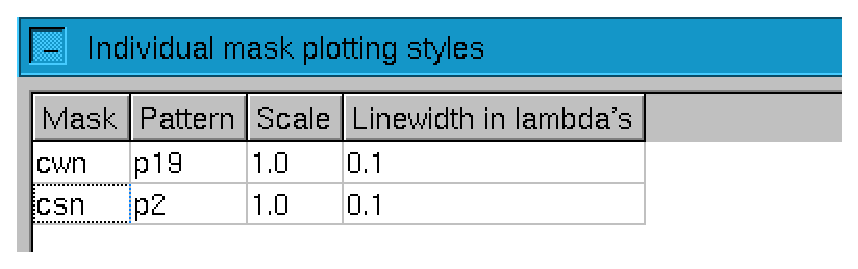
\includegraphics[width=7cm]{./figures/ex_section.eps}
\caption{Section example result.}
\end{center} \end{figure}


\subsection{Components in a scrollframe context}
A scrollframe component is useful primarily inside tabpages. The scrollframe
will then occupy the entire tabpage area, maximizing the area available to the
components inside the frame. Using multiple scrollframes inside a tabpage or
nesting scrollframes is not allowed. This is a limitation in the current
scrollframe implementation. The resulting behaviour is undefined.

There are no properties for the scrollframe itself, because the scrollframe is
not really a visible widget and the behaviour is fixed. Future versions could
implement some properties to influence the behaviour. Examples could be
properties to influence the used layout mechanism (horizontal/vertical) or
child alignment (for example to center or right-justify the widgets instead of
the current left justification).

%%%\small
%%%\begin{center}
%%%\begin{tabularx}{\textwidth}{|l|l|X|}
%%%  \hline
%%%  \multicolumn{3}{|X|}{\textsf{List of accepted child components}} \\
%%%  \hline
%%%
%%%  \multicolumn{3}{|X|}{Child component type: \texttt{real, integer, identifier, string, spreadsheet}} \\
%%%  \hline
%%%  &  \textsf{Property} & \textsf{Description} \\
%%%  \cline{2-3}
%%%  & \texttt{hint} & The value of this property will be shown as a hint text as the mouse ``hovers'' over the widget. The hint text can be split over multiple lines by inserting $\backslash$n at the right places. \\
%%%  \cline{2-3}
%%%  & \texttt{default} & The value of this property will be used as the default value to display in the widget (ignored for spreadsheets). \\
%%%  \cline{2-3}
%%%
%%%  & \multicolumn{2}{|X|}{Ignored properties: \mbox{\texttt{title, align, pixmap, option, unit}}} \\
%%%  \cline{2-3}
%%%  & \multicolumn{2}{|X|}{Forbidden properties: \texttt{adddatafrom}} \\
%%%  \hline
%%%
%%%  \multicolumn{3}{|l|}{Child component type: \texttt{dropdown}} \\
%%%  \hline
%%%  &  \textsf{Additional properties} & \textsf{Description} \\
%%%  \cline{2-3}
%%%  & \texttt{adddatafrom} & The value of this property is a reference to the data source. The data from the source is used as the entries in this dropdown. \\
%%%  \cline{2-3}
%%%  & \texttt{default} & The value of this property must be the name of an \texttt{item} child of the dropdown. \\
%%%  \cline{2-3}
%%%
%%%  & \multicolumn{2}{|X|}{Ignored properties: \mbox{\texttt{align, pixmap, option}}} \\
%%%  \cline{2-3}
%%%
%%%
%%%  \multicolumn{3}{|l|}{Child component type: \texttt{section}} \\
%%%  \hline
%%%  &  \textsf{Properties} & \textsf{Description} \\
%%%  \cline{2-3}
%%%  & \texttt{title} &  The value of this property is displayed in the title bar of the section. \\
%%%  \cline{2-3}
%%%  & \texttt{hint} &  The value of this property will be shown as a hint text as the mouse ``hovers'' over the section. The hint text can be split over multiple lines by inserting $\backslash$n at the right places.\\
%%%  \cline{2-3}
%%%  & \texttt{pixmap} &  The value of this property is the filename of a file containing a pixmap. The filename must be given relative to the \texttt{ICONPATH} specified at the top of the configuration file. The \texttt{ICONPATH} can only contain a single path (for example: \texttt{ICONPATH = "\$(ICDPATH)/lib/spock"}. Environment variables are expanded.)\\
%%%  \cline{2-3}
%%%
%%%  & \multicolumn{2}{|X|}{Ignored properties: \mbox{\texttt{default, align, unit, option}}} \\
%%%  \cline{2-3}
%%%  & \multicolumn{2}{|X|}{Forbidden properties: \texttt{adddatafrom}} \\
%%%  \hline
%%%
%%%  \hline
%%%  \multicolumn{3}{|X|}{Using forbidden properties or unlisted component types as children will result in undefined behaviour.} \\
%%%  \hline
%%%\end{tabularx}
%%%\end{center}
%%%\normalsize

\paragraph{Example:}
\begin{alltt}
scrollframe \emph{element_def} \{
    section \emph{units};
    section \emph{conductors};
    section \emph{fets};
    section \emph{bjts};
    section \emph{connects};
    section \emph{contacts};
    section \emph{capacitances};
\}
\end{alltt}
\noindent This example shows how some section widgets are placed inside a
scrollframe.

\begin{figure}[h!] \begin{center}
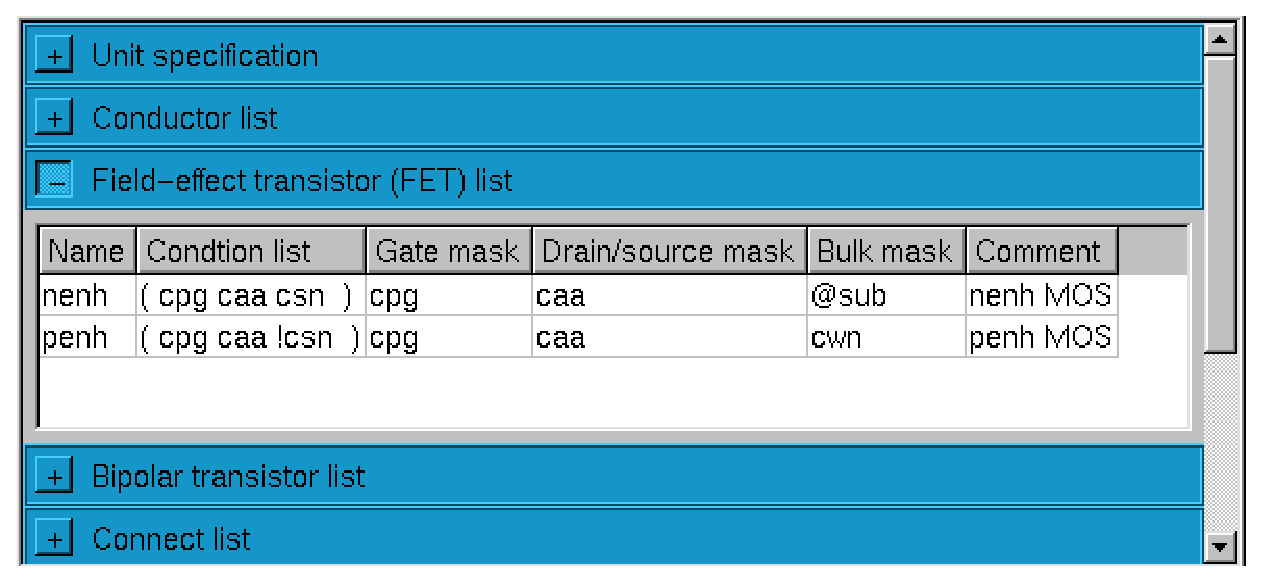
\includegraphics[width=7cm]{./figures/ex_scrollframe.eps}
\caption{Scrollframe example result.}
\end{center} \end{figure}


\subsection{Components in a tabpage context}
Tabpage components will become the tabpages in the user interface. A tabpage
must therefore have a title to distinguish it from the other tabpages.

%\begin{PropTable}
% \verb=title=       & Use the \verb=title= property to set the tabpage label. \\
% \verb=hint=        & Sets the hint text that will be displayed when the mouse
%                      hovers over the tabpage label.
%\end{PropTable}

%%%\small
%%%\begin{center}
%%%\begin{tabularx}{\textwidth}{|l|l|X|}
%%%  \hline
%%%  \multicolumn{3}{|X|}{\textsf{List of accepted child components}} \\
%%%  \hline
%%%
%%%  \multicolumn{3}{|X|}{Child component type: \texttt{real, integer, identifier, string, spreadsheet}} \\
%%%  \hline
%%%  &  \textsf{Property} & \textsf{Description} \\
%%%  \cline{2-3}
%%%  & \texttt{hint} & The value of this property will be shown as a hint text as the mouse ``hovers'' over the widget. The hint text can be split over multiple lines by inserting $\backslash$n at the right places. \\
%%%  \cline{2-3}
%%%  & \texttt{default} & The value of this property will be used as the default value to display in the widget (ignored for spreadsheets). \\
%%%  \cline{2-3}
%%%
%%%  & \multicolumn{2}{|X|}{Ignored properties: \mbox{\texttt{title, align, pixmap, option, unit}}} \\
%%%  \cline{2-3}
%%%  & \multicolumn{2}{|X|}{Forbidden properties: \texttt{adddatafrom}} \\
%%%  \hline
%%%
%%%  \multicolumn{3}{|l|}{Child component type: \texttt{dropdown}} \\
%%%  \hline
%%%  &  \textsf{Additional properties} & \textsf{Description} \\
%%%  \cline{2-3}
%%%  & \texttt{adddatafrom} & The value of this property is a reference to the data source. The data from the source is used as the entries in this dropdown. \\
%%%  \cline{2-3}
%%%  & \texttt{default} & The value of this property must be the name of an \texttt{item} child of the dropdown. \\
%%%  \cline{2-3}
%%%
%%%  & \multicolumn{2}{|X|}{Ignored properties: \mbox{\texttt{align, pixmap, option}}} \\
%%%  \cline{2-3}
%%%
%%%
%%%  \multicolumn{3}{|l|}{Child component type: \texttt{section}} \\
%%%  \hline
%%%  &  \textsf{Properties} & \textsf{Description} \\
%%%  \cline{2-3}
%%%  & \texttt{title} &  The value of this property is displayed in the title bar of the section. \\
%%%  \cline{2-3}
%%%  & \texttt{hint} &  The value of this property will be shown as a hint text as the mouse ``hovers'' over the section. The hint text can be split over multiple lines by inserting $\backslash$n at the right places.\\
%%%  \cline{2-3}
%%%  & \texttt{pixmap} &  The value of this property is the filename of a file containing a pixmap. The filename must be given relative to the \texttt{ICONPATH} specified at the top of the configuration file. The \texttt{ICONPATH} can only contain a single path (for example: \texttt{ICONPATH = "\$(ICDPATH)/lib/spock"}. Environment variables are expanded.)\\
%%%  \cline{2-3}
%%%
%%%  & \multicolumn{2}{|X|}{Ignored properties: \mbox{\texttt{default, align, unit, option}}} \\
%%%  \cline{2-3}
%%%  & \multicolumn{2}{|X|}{Forbidden properties: \texttt{adddatafrom}} \\
%%%  \hline
%%%
%%%  \multicolumn{3}{|l|}{Child component type: \texttt{section}} \\
%%%  \hline
%%%  & \multicolumn{2}{|X|}{The scrollframe is not a visible widget. It does not use any properties.} \\
%%%  \cline{2-3}
%%%  & \multicolumn{2}{|X|}{Ignored properties: \mbox{\texttt{title, hint, default, align, unit, pixmap, option}}} \\
%%%  \cline{2-3}
%%%  & \multicolumn{2}{|X|}{Forbidden properties: \texttt{adddatafrom}} \\
%%%  \hline
%%%
%%%  \hline
%%%  \multicolumn{3}{|X|}{Using forbidden properties or unlisted component types as children will result in undefined behaviour.} \\
%%%  \hline
%%%\end{tabularx}
%%%\end{center}
%%%\normalsize


\paragraph{Example:}
\begin{alltt}
tabpage \emph{getepslay_tab} \{
    title("Postscript plot settings");
    scrollframe \emph{getepslay_frame} \{
        section \emph{getepslay_preamble};
        section \emph{getepslay_body};
    \}
\}
\end{alltt}

\subsection{Overview of combinations}
Table \ref{tab:language:overview} lists the existing relationships between
component types in a certain context and the properties that can be used. Note
that the table lists the \emph{implemented} relationships, not the
\emph{possible} relationships. Additional sensible relationships could be
implemented in a future version of the application.

The numbers in the table refer to the explanations given below. Some numbers
are followed by a letter. The letter \texttt{r} indicates that the property is
required. If these properties are not specified the behaviour of the
application is undefined. The letter \texttt{F} indicates that it is forbidden
to specify that property. If the property is specified anyway, the behaviour of
the application is undefined.

The label \texttt{r.i.s.i.} stands for real, integer, string or identifier. The
row is valid for each of these component types. The combobox type is missing,
but the properties and contexts listed for the dropdown are identical to the
ones listed for the combobox.

If a combination of a component and a context is not listed in the table, the
behaviour resulting from this combination is undefined.

\actd{title1} \actd{title2} \actd{title3} \actd{title4} \actd{hint1}
\actd{hint2} \actd{hint3} \actd{default1} \actd{default2} \actd{align1}
\actd{adddata1} \actd{adddata2} \actd{unit1} \actd{pixmap1} \actd{option1}
\begin{center} \begin{table}
\caption{Combinations of components and properties in a context.}
\label{tab:language:overview}
\small
\begin{tabularx}{\textwidth}{|l|X|c|c|c|c|c|c|c|c|c|c|}
 \hline
 \textsf{Context} & \textsf{Acceptable component types} & \rotated{title} & \rotated{hint} & \rotated{default} & \rotated{align} & \rotated{adddatafrom} & \rotated{unit} & \rotated{pixmap} & \rotated{option} \\
 \hline
 dropdown    & item      & \TR[r]{title1} & & & & F & & & \\ \hline
 spreadsheet & r.i.s.i   & \TR[r]{title2} & & \R{default1} & \R{align1}& F & & & \\ \cline{2-10}
%             & integer   & \TR[r]{title2} & & \R{default1} & \R{align1}& F & & & \\ \cline{2-10}
%             & string    & \TR[r]{title2} & & \R{default1} & \R{align1}& F & & & \\ \cline{2-10}
%             & identifier& \TR[r]{title2} & & \R{default1} & \R{align1}& F & & & \\ \cline{2-10}
             & color     & \TR[r]{title2} & & \R{default1} & & F & & & \\ \cline{2-10}
             & dalistyle & \TR[r]{title2} & & \R{default1} & & F & & & \\ \cline{2-10}
             & conditionlist & \TR[r]{title2} & & & \R{align1} & \TR[r]{adddata1} & & & \R{option1} \\ \hline
 section     & r.i.s.i.  & & \R{hint1} & \R{default1} &  &  F & & & \\ \cline{2-10}
             & dropdown  & & \R{hint1} & \R{default1} &  &  \R{adddata2} & & & \\ \cline{2-10}
             & spreadsheet & & \R{hint1} & & & F & &  & \\ \hline
 paramlist   & r.i.s.i   & \R{title3} & \R{hint2} & \R{default1} & & F & \R{unit1} &  & \\ \cline{2-10}
             & dropdown  & \R{title3} & \R{hint2} & \R{default2} & & \R{adddata2} & \R{unit1} & &  \\ \cline{2-10}
             & spreadsheet & \R{title3} & \R{hint2} & & & F & \R{unit1} & &  \\ \hline
 scrollframe & r.i.s.i.  & & \R{hint1} & \R{default1} & & F & & &  \\ \cline{2-10}
             & dropdown  & & \R{hint1} & \R{default2} &  &  \R{adddata2} & & & \\ \cline{2-10}
             & spreadsheet & & \R{hint1} & & & F & & &  \\ \cline{2-10}
             & section   & \R{title4}& \R{hint3} & & & & & \R{pixmap1} & \\ \hline
 tabpage     & r.i.s.i.  & & \R{hint1} & \R{default1} & & F  & & & \\ \cline{2-10}
             & dropdown  & & \R{hint1} & \R{default2} &  &  \R{adddata2} & & & \\ \cline{2-10}
             & spreadsheet & & \R{hint1} & & & F & & &   \\ \cline{2-10}
             & section   & \R{title4}& \R{hint3} & & & & & \R{pixmap1} & \\ \cline{2-10}
             & scrollframe & & & & & & & & \\ \hline
\end{tabularx}
\normalsize \end{table} \end{center}

The numbers in Table \ref{tab:language:overview} are explained below:\small
\begin{itemize}
\item[\R{title1}] The value of this property will be used as the text of the corresponding entry in the dropdown.
\item[\R{title2}] The value of this property will be used as the title of the corresponding column in the spreadsheet.
\item[\R{title3}] The value of this property will be used as the label in the first column of the parameter list.
\item[\R{title4}] The value of this property will be used as the title displayed in the section bar.
\item[\R{hint1}] The value of this property will be shown as a hint text as the mouse ``hovers'' over the widget. The hint text can be split over multiple lines by inserting $\backslash$n at the right
places. Quotation marks can be inserted with
\texttt{$\backslash$"}.
\item[\R{hint2}] The value of this property will be shown as a hint text as the mouse ``hovers'' over the widget in the second column. The hint text can be split over multiple lines by inserting $\backslash$n at the right
places. Quotation marks can be inserted with
\texttt{$\backslash$"}.
\item[\R{hint3}] The value of this property will be shown as a hint text as the mouse ``hovers'' over the section bar. The hint text can be split over multiple lines by inserting $\backslash$n at the right
places. Quotation marks can be inserted with
\texttt{$\backslash$"}.
\item[\R{default1}] The value of this property will be used as default value to display in the spreadsheet cells of this column.
\item[\R{default2}] The value of this property must be the name of one of the
child items. This item will be shown as the default value in the
dropdown/combobox.
\item[\R{align1}] The value of this property can be \texttt{left, right} or \texttt{center}. The spreadsheet column will be aligned accordingly.
\item[\R{adddata1}] This property accepts two values. Both values must be
identifiers that can be unambiguously resolved. The data referenced by the
first (required) identifier will be used for the layer names in the
conditionlist. The second (optional) identifier references the layer
descriptions.
\item[\R{adddata2}] This property accepts one or more values. Each value is an
identifier that can be unambiguously resolved. The data referenced by each
identifier will be concatenated and the result will become the entries in the
dropdown/combobx.
\item[\R{unit1}] The value of this property will be used as the label in the third column of the parameter
list, after the input field.
\item[\R{pixmap1}] The value of this property is the filename of a file
containing a pixmap. The filename must be given relative to the
\texttt{ICONPATH} specified at the top of the configuration file. The
\texttt{ICONPATH} can only contain a single path (for example: \texttt{ICONPATH
= "\$(ICDPATH)/lib/spock"}. Environment variables are expanded and can be
specified \texttt{Makefile} style: between parenthesis preceded by a \$.)
\item[\R{option1}] This property value must be either \texttt{extended} or
\texttt{noextended}. If \texttt{extended} is specified, the conditionlist
editor is shown with three columns: `one side', `tile' and `other side'. If
\texttt{noextended} is specified, only the `tile' column will be displayed.
\end{itemize}
\normalsize


%%%%%%%%%%%%%%%%%%%%%%%%%%%%%%%%%%%%%%%%%%%%%%%%%%%%%%%%%%%%%%%%%%%%%%%%%%%%%
\section{Language overview for generators} \label{sect:language:generatorref}
This section will present and explain the generator specification in the
configuration file language. The generator specification is put into an
expression tree that evaluates to the contents of the technology files.

The generator component is described first in Section
\ref{sect:language:generator_components}. After that, the use of value mappings
is explained in Section \ref{sect:language:valmaps}. The sections following
Section \ref{sect:language:valmaps} describe the expressions that can be used
inside the \verb=generate= context.

\subsection{Generator components} \label{sect:language:generator_components}
The generator components are specified the same way as the other components in
the configuration file. An example was already given in Section
\ref{sect:language:generators_intro} and is repeated below:
\begin{alltt}
generator \emph{maskdata_gen} \{
    filename("maskdata");
    title("Maskdata file");

    generate \{
        "# Automatically generated file. Do not edit.\(\backslash\)n"
        "number_of_rows:\t" maksdata_sheet.numrows "\(\backslash\)n"
        "#############################################\(\backslash\)n"
    \}
\}
\end{alltt}
The generator type component uses a language construction similar to the other
component types. Like the other component types, properties can be used and the
declaration syntax is the same. However, this component is not translated into
a user interface element. More importantly, additional language constructions
can be used inside the generator component.

The additional language constructions that can be used are the value mappings
and the \verb=generate= statement. The expressions describing the technology
file format must be put inside the generate statement

\begin{PropTable}[The properties supported by the generator component:]
 \verb=title=       & Use the \verb=title= property to set a short descriptive name
                      for the generator. This descriptive name is used in several places in the application, for example in the technology file generation dialog box.\\
 \verb=filename=    & The filename of the technology file to generate. This is
                      only the filename, not the path. The path is specified by
                      the user in the user interface.
\end{PropTable}

If the \verb=title= property is not specified, the description is an empty
string. If the filename property is not specified, the behaviour of the
application is undefined.

\subsection{Value mappings}\label{sect:language:valmaps}
Besides the properties, the generator component supports value mappings. Value
mappings allow the substitution of text used in the \verb=dropdown= and
\verb=combobox= items to a string in the technology file. This allows the use
of a descriptive text in the user interface and a specialized string in the
generated technology file. An example of the construction is given below. The
\verb=dropdown= used in the substitution is also shown to illustrate the
mechanism.

\begin{alltt}
define combobox \emph{def_carr_type} \{
    item \emph{n} \{ title("n doped conductor"); \}
    item \emph{p} \{ title("p doped conductor"); \}
    item \emph{m} \{ title("metal"); \}
    default(\emph{m});
\}

map \emph{def_carr_type} \{
    n = "n";
    p = "p";
    m = "m";
\}
\end{alltt}

The value mapping could of course be extended into a more general mechanism
that allows arbitrary substitutions. This would increase the flexibility of the
generators.

Looking at the example above, one could argue that the identifier name could be
used as a substitution. This has however, as a disadvantage that it would not
be possible to substitute a text that is not an identifier, meaning spaces or
other special symbols could not be used.

\subsection{Literal text}
Use quotation marks to generate literal text. Literal text may contain tabs and
newlines like in C++ using \verb=\t= and \verb=\n=. If quotation marks are
needed they too can be escaped (\verb=\"=). Concatenation of strings can be
used to span long literals over several lines. This is illustrated in the
example below.

\begin{verbatim}
generate {
    "Literal text must be placed between quotation marks (\").\n"
    "\n and \t can be used like in C++. Bordering "
    "literals "   "are "   "concatenated in the output of "
    "the generator."
}
\end{verbatim}

\subsection{Identifier substitution}
To place values in the generator output we can use the name of any identifier
in the user interface specification. The identifier will be replaced with the
value that is currently entered in the applications' user interface.

\begin{verbatim}
generate {
    "The value of getepslay_pl.mask_order is: "
    getepslay_pl.mask_order "\n"
}
\end{verbatim}

Some component types do not generate any output. These are usually types that
contain other components like the scrollframe and the section components.

\bigskip \noindent
In some cases, not the actual value of identifier is required but some other
property. This is achieved by the use of fields. For example, to generate the
number of layers \verb=maskdata_sheet[numrows]= could be used. The field is
specified between square brackets after the identifier name. The currently
supported fields are listed in Table \ref{tab:language:fieldsupport}

Besides the identifiers present in the user interface specification, there is
also a special identifier called
\verb=application=. This identifier can be used to retrieve values from the
application that are not present in the user interface specification.
\verb=application= is a reserved word. If \verb=application= is inadvertently used as an identifier, the parser will exit
with an error.

\begin{table}[h] \begin{center}
\caption{Supported fields:}
\label{tab:language:fieldsupport}
\begin{tabularx}{\textwidth}{l|l|X}
\hline
 \textsf{Component type} & \textsf{Fields} & \textsf{Description} \\
\hline
\texttt{spreadsheet} & \texttt{numrows} & Is replaced with the number of rows present in the spreadsheet. \\
\texttt{dalistyle}   & \texttt{fill} & Is replaced with the selected dali fill number \\
                     & \texttt{clr}  & Is replaced with the selected dali color number \\
\texttt{application} & \texttt{time} & Is replaced with the current time \\
                     & \texttt{date} & Is replaced with the current date \\
                     & \texttt{processname} & Is replaced with name of the process being generated \\
                     & \texttt{processdesc} & Is replaces with a description of the process being generated \\
\hline
\end{tabularx}
\end{center}\end{table}

\subsection{Number addition and subtraction}
Simple addition and subtraction is also supported. For example:
\begin{verbatim}
generate {
    "The number of layers + 1 = " maskdata_sheet[numrows] + 1
}
\end{verbatim}

The type of the result depends on the type of the operands. Two integer
operands will result in an integer but two reals or a real and a integer will
result in a real.

\subsection{Loops}
For spreadsheets it is necessary to be able to loop over the rows or all values
present in a column of a spreadsheet. To support this, a \verb=foreach= loop is
introduced. The foreach loop has two forms. The first form loops over the rows
and has no loop variable:

\begin{verbatim}
foreach(fets.fets_sheet, row) {
   "    " name ":" cond_list ":" mask_g " " mask_ds
   ":" mask_b " # " comment "\n"
}
 "\n"
\end{verbatim}
\verb=fets.fets_sheet= is a hint context. The identifiers inside the loop body
are first resolved using this context. If that yields no results a normal
disambiguation is tried.

\bigskip \noindent
Besides iterating over spreadsheet rows it is also possible to iterate over the
values present in a column. Each value in that column is enumerated exactly
once:

\begin{alltt}
foreach \$t (conductors_sheet, cond_type) {
    "conductor " \$t "\(\backslash\)n"
}
\end{alltt}

Again, the first argument between the brackets is the hint context. The second
argument is an identifier that is a spreadsheet column. All values in that
column will be enumerated.

The loop variable can be used (here \texttt{\$t}) to access the current value
of an iteration. This makes it possible to nest loops. Each loop variable
corresponds to the current iteration values of each of the loops.

If the \verb=cond_type= column contained the values a, b, a, c, d, and a, the
result would be:
\begin{verbatim}
 conductor a
 conductor b
 conductor c
 conductor d
\end{verbatim}

For an example of some more difficult nested loops please take a look at the
sample \verb=spock.uis= configuration file in Appendix \ref{chapt:samplespock}.

\subsection{Conditionals}
In some cases it is necessary to generate a piece of text conditionally. To be
able to do this, a conditional statement is needed. This is provided by the
\verb=if= statement.

\begin{alltt}
foreach \$t (cap_sheet, cap_type) \{
   foreach \$s (cap_sheet, subtype) \{
        \$t " capacitances " \$s ":\(\backslash\)n"
        "#\(\backslash\)tname:condition_list:type:mask1 [mask2]:capacitivity\(\backslash\)n"
        foreach(capacitances.cap_sheet, row) \{
           if (cap_type == \$t) \{
               if (subtype == \$s) \{
                   "\(\backslash\)t" name ":" cond_list ":" mask_1 " " mask_2 ":" capacitivity "\(\backslash\)t\(\backslash\)t# " comment "\(\backslash\)n"
               \}
           \}
        \}
        "\(\backslash\)n"
   \}
\}
\end{alltt}

%\begin{alltt}
%if (space_params.min_coup_cap != "") \{
%    "min_coup_cap "  space_params.min_coup_cap  "\(\backslash\)n"
%\}
%\end{alltt}

\bigskip \noindent
The possible conditional statements are limited to equal or not equal. The
operators for this are \verb|==| and \verb|!=|. Support for additional
operators could easily be implemented in a future version.

%%%%%%%%%%%%%%%%%%%%%%%%%%%%%%%%%%%%%%%%%%%%%%%%%%%%%%%%%%%%%%%%%%%%%%%%%%%%%
\section{Recommended language extensions} \label{sect:language:extensions}
Language extensions can be grouped into two categories:
\begin{enumerate}
\item extensions to the language itself
\item extensions in the form of new types and properties
\end{enumerate}

\subsection{Language extensions}
The configuration file language is quite complete in functionality. However,
some common language constructions seen in other languages are not yet
possible.
\begin{itemize}
\item \textbf{Operators\\ } Currently only + and -- are supported. It is of
course possible to add multiplication (*), division (/) and more math-like
functions like powers (\verb=^=) and perhaps even \verb=sin()= and
\verb=cos()=. This depends on the need for them of course.
\item \textbf{Conditionals\\ } The conditional \verb=if= statement could be
extended with \verb=else= support and additional comparisons like less then and
greater then (\verb=<= and \verb=>=).
\item \textbf{Loops\\ } The \verb=foreach= loop construction provided is
sufficient for simple loops. It could be useful to implement additional loop
structures like \verb=do-while= or \verb=while-do=.
\item \textbf{Value substitition\\ } The value substitution mechanism provided
by the value maps could be extended to a more general substitution mechanism
that can substitute any string for another.
\item \textbf{Perl\\ } It is also possible to embed perl into the application.
The expressions describing the technology file formats could become a block of
perl source.

This mechanism could even be extended to the complete configuration file.
Special perl functions internally defined by the application could then be
called in the configuration file to build the trees.

The disadvantage of using perl is the addition of a dependency to the
application and the possible compilation difficulties on different platforms.
\end{itemize}

\subsection{New types and properties}
Besides extensions to the language itself, it is also possible to add new types
and properties to the language.
\begin{itemize}
\item \textbf{Layout control\\ } It is possible to add properties or components
that use Qt's widget layout mechanism. There would be more control over the
arrangement of the components in this case (For example a \verb=vbox{}= and
\verb=hbox{}= component that layout their children vertically or horizontally).
\item \textbf{More editors\\ } The addition of types would allow more special
purpose editors like the condition list editor and the dali color picker. A
capacitance value generating editor for example (that could be used to generate
the capacitances in the element definition files). Another editor could be a
``pattern picker'' for the fill patterns used by \verb=getepslay=.
\item \textbf{Additional properties\\ } Additional properties can also be very
useful. For example:
    \begin{itemize}
    \item The Qt \verb=whatis= mechanism could be implemented so a \verb=whatis=
    property can be added. This would enhance the context sensitive help
    available to the end user.
    \item More properties that control the looks of a component could be added,
    for example a \verb=font= property that influences the font used in the
    component or a \verb=background= property to set the background color of a
    component.
    \end{itemize}
\item \textbf{Property warnings\\ } Warnings or errors should be given if
required properties are missing or if forbidden or ignored properties are used
\item \textbf{Better default values\\ } If properties are unspecified but can
be used in a certain context, sensible defaults could be chosen. For example,
if the \verb=title= property of generator component is not given it could use
the filename specified in the \verb=filename= property.
\item \textbf{Better conditional output\\ } In some cases (a good example is the
parameter list) the file generation could be simplified if some built-in
construction is available for empty parameter values. This would avoid long
lists of \verb=if= constructions. This could be implemented by some general
mechanism or a parameter specific mechanism.
\end{itemize}
